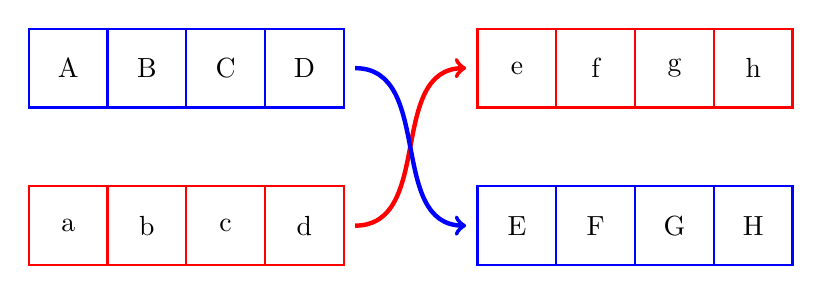
\begin{tikzpicture}[ultra thick]
	
	%nodes in the red genome have names of the form r1, r2 ...
	%nodes in the blue genome have names of the form b1,br2 ...


	\def\xskip{1.7}
	\def\xArrowSkip{0}
	\def\yskip{-2}
	\def\halfSquare{0.5}
	\def\leftListLength{4}
	\def\control{1.15}
	\def\mysquare{+(-\halfSquare , -\halfSquare  ) rectangle +(\halfSquare ,\halfSquare )}

	%blue, upper left
	\foreach \label/\position in {A/1, B/2,  C/3,  D/4}
   {
		\draw [blue, thick] (\position,0) \mysquare;
		\node (b\label) at (\position,0) {\label};
   }
	
	%red, lower left
\foreach \label/\position in {a/1,  b/2,  c/3,  d/4}
   {
		\draw [red, thick] (\position,\yskip) \mysquare;
		\node (r\label) at (\position, \yskip) {\label};
   }

	%red. upper right
\foreach \label/\position in {e/5,  f/6,  g/7,  h/8}
   {
		\draw [red, thick] (\xskip + \position,0) \mysquare;
		\node (r\label) at (\xskip + \position, 0) {\label};
   }


	%blue. lower right
\foreach \label/\position in {E/5,  F/6,  G/7,  H/8}
   {
		\draw [blue, thick] (\xskip + \position,\yskip) \mysquare;
		\node (b\label) at (\xskip + \position, \yskip) {\label};
   }

	%Arrows

	\node (redArrowStart) at (\leftListLength * 2 * \halfSquare + \halfSquare + \xArrowSkip ,\yskip){};
	\node (blueArrowStart) at (\leftListLength * 2 * \halfSquare + \halfSquare + \xArrowSkip ,0){};
	\node (redArrowEnd) at (\leftListLength * 2 * \halfSquare + \halfSquare + \xskip - \xArrowSkip ,0){};
	\node (blueArrowEnd) at (\leftListLength * 2 * \halfSquare + \halfSquare + \xskip - \xArrowSkip ,\yskip){};

	\draw [->, red, ultra thick] (redArrowStart)  .. controls +(right: \control) and +(left: \control) ..  (redArrowEnd);
	\draw [->, blue, ultra thick] (blueArrowStart)  .. controls +(right: \control) and +(left: \control) ..  (blueArrowEnd);

	
	%for orientation: find the red ball
	%\draw [fill=red] (\leftListLength * 2 * \halfSquare + \halfSquare + \xArrowSkip ,\yskip) circle (0.1);

\end{tikzpicture}